
\documentclass[a4paper]{jpconf}
\usepackage{graphicx}
% \usepackage{color}
% \usepackage{array}
% \usepackage{enumerate}

% To create a graphic:
% 1) save your image as a 1024x1024 png/gif/bmp
% 2) convert to pdf (install ImageMagick, then 'convert FileIn.png FileOut.pdf')
% 3) to resize the image, if needed, 'convert FileIn.png -resize 66% FileOut.pdf' etc
% N.B. if the input and output files have the same base name, LaTeX will prefer to take the png
% over the pdf, which is probably not what you want. Make sure the files have different names!
%\begin{figure}[htp]
%\centering
%\includegraphics{file-basename}
%\caption{figure caption blah blah}\label{fig:figure-ref}
%\end{figure}

\begin{document}
\title{Monitoring data transfer latency in CMS computing operations}

\author{D~Bonacorsi$^1$, T~Diotalevi$^1$, N~Magini$^2$, A~Sartirana$^3$, M~Taze$^4$, and T~Wildish$^5$}

\address{$^1$ University of Bologna}
\address{$^2$ Fermi National Accelerator Laboratory}
\address{$^3$ Ecole Polytechnique of Paris}
\address{$^4$ Cukurova University}
\address{$^5$ Princeton University}

\ead{Daniele.Bonacorsi@bo.infn.it, nicolo.magini@cern.ch, meric.taze@cern.ch, sartiran@llr.in2p3.fr, Tony.Wildish@cern.ch}

\begin{abstract}

During the first LHC run, the CMS experiment collected tens of
Petabytes of collision and simulated data, which need to be
distributed among dozens of computing centres with low latency in
order to make efficient use of the resources. While the desired level
of throughput has been successfully achieved, it is still common to
observe transfer workflows that cannot reach full completion in a
timely manner due to a small fraction of stuck files which require
operator intervention.

For this reason, in 2012 the CMS transfer management system, PhEDEx,
was instrumented with a monitoring system to measure file transfer
latencies, and to predict the completion time for the transfer of a
data set. The operators can detect abnormal patterns in transfer
latencies while the transfer is still in progress, and monitor the
long-term performance of the transfer infrastructure to plan the data
placement strategy.

Based on the data collected for one year with the latency monitoring
system, we present a study on the different factors that contribute to
transfer completion time. As case studies, we analyze several typical
CMS transfer workflows, such as distribution of collision event data
from CERN or upload of simulated event data from the Tier-2 centres to
the archival Tier-1 centres. For each workflow, we present the typical
patterns of transfer latencies that have been identified with the
latency monitor.

We identify the areas in PhEDEx where a development effort can reduce
the latency, and we show how we are able to detect stuck transfers
which need operator intervention. We propose a set of metrics to alert
about stuck subscriptions and prompt for manual intervention, with the
aim of improving transfer completion times.

\end{abstract}

\section{Introduction}
\label{sec:intro}

The CMS experiment \cite{CMS} at the LHC accelerator is concluding the
first Long Shutdown (LS1) after a successful first run of data taking
(Run-1), with Run-2 starting in Summer 2015. In the original CMS
Computing model \cite{CompModel}, one of the main concepts of the data
management \cite{DataMgmt} was that jobs go where the data is, and no
data moves in response to job submissions. In such model, the
importance of adequate policies and tools for data placement is
vital. Over the years, this motivated the CMS Computing project to
design, build and operate a robust and reliable solution to perform
transfers of massive volumes of data among computing centres of the
Worldwide LHC Computing Grid (WLCG) \cite{WLCG,WLCG2}, called PhEDEx
\cite{PhEDEx1, PhEDEx2, PhEDEx3, PhEDEx4}. PhEDEx is a reliable and
scalable dataset replication system based on a central database on an
Oracle instance running at CERN and a set of highly specialised,
loosely-coupled, stateless software agents distributed at sites. In
production for CMS since more than 10 years, PhEDEx moved 150 PB
during Run-1, and it is currently moving about 2.5 PB per week among
about 60 sites.  The PhEDEx design aims at providing the highest
possible transfer completion rate, despite possible infrastructural
unreliabilities, achieved via intelligent fail-over tactics and
automatic retrials. During the several years of its operations,
including the first LHC data taking period (Run-1) and the first LHC
Long Shutdown (LS1), a large set of data concerning the latencies
observed in all transfers between all Tiers has been collected. The
study of this data set is allowing a categorisation of the different
root sources of such latencies and shaping the strategy to attach this
problem and increase the overall performance of the PhEDEx system.

\section{Instrumenting PhEDEx to collect latency data}
\label{sec:instrumenting}

The atomic unit for transfer operations in PhEDEx is the file block:
an arbitrary group of O(100-1000) files in the same dataset.  To
achieve scalability, PhEDEx doesn't keep a permanent record of the
states of individual files: all information is aggregated at the level
of block after transfers are completed.

This level of detail is sufficient for replica location, but it is not
enough to identify problems that increase latency in block transfers:
for example, there is no way to distinguish between the case of a
high-latency transfer proceeding at a low regular rate, and the case
of a transfer for which the latency is dominated by a few stuck files
in the ``transfer tail''.

For this reason, in 2012 we instrumented the central agents of PhEDEx
with a detailed latency monitoring system \cite{phedexlatency},
collecting file-level information on transfers in historical
monitoring tables to complement block-level information, and providing
corresponding Data Service APIs to retrieve the monitoring data for
further analysis.

The BlockAllocator agent that is responsible for monitoring
subscriptions records the timestamps of the main events related to
block completion in the t\textunderscore dps\textunderscore
block\textunderscore latency table: the time when the block was
subscribed and the time when the last file in the block was
successfully replicated at destination.  The difference between these
two timestamps can be defined as the total latency for block
replication as experienced by users, which may also include time spent
while the subscription was manually suspended by an operator.  In this
case, the agent also measures and records in the table the time
elapsed during the suspension, and subtracting this value from the
total latency we measure what we define as the ``PhEDEx latency'',
i.e. introduced by PhEDEx itself and the underlying transfer
infrastructure rather than human intervention.


The FilePump agent responsible for collecting the results of transfer
tasks records a summary of the transfer history of each file in the
block in the t\textunderscore xfer\textunderscore file\textunderscore
latency table, including the time when the file was first activated
for routing, the time of the first transfer attempt and of the final
successful transfer attempt, the number of transfer attempts needed
for the file to arrive at destination, as well as the source node of
the first and last transfer attempts (which may be different if the
transfer was rerouted).



For performance reasons, the entries in these live tables are archived
to historical tables after the transfer is completed: file-level
statistics into t\textunderscore log\textunderscore
file\textunderscore latency, which is eventually cleaned up after 30
days, and block-level statistics into t\textunderscore
log\textunderscore block\textunderscore latency, in which they are
kept indefinitely and integrated with additional events related to
block completion:
\begin{itemize}
\item the time when the first file in the block was routed for transfer
\item the time when the first file in the block was successfully
  replicated at destination
\item the times when 25\%/50\%/75\%/95\% of the files in the block
  were replicated at destination
\item the time when the last file in the block was successfully
  replicated at destination
\end{itemize}
In addition, we record the total number of transfer attempts needed to
transfer all files in the block, as well as the source node for the
majority of files in the block.

\section{Cleaning data and defining variables}

In the last two years, thanks to the instrumentation detailed in the
previous session, the PhEDEX system collected records about the
latency of roughly 3 million block subscriptions.  This data include
several useful informations:

\begin{itemize}
\item block informations: block, number of files, size, timestamps of
    the block opening and closing;
\item subscription informations: destination site, custodiality flag,
    total time of suspension, creation date of the subscription,
    priority;
\item source sites informations: site from which most files where
    transferred and number of files transferred from this site;

\item informations about the transfer execution: timestamps of the first
    request, the first transfer, the 25\%/50\%/75\%/95\% completion and of
    the last transfer. The total number of transfers attempts.
\end{itemize}

This huge amount of records represents the raw input of our
analysis. Before starting the actual analytic work, however, this set
of data has to undergo some cleaning and processing steps in order to
remove the items of no interest and define useful derived observables.

First of all we cleaned ill defined data, that is records with missing
or inconsistent entries. These are mostly issued from test transfers
and represent roughly the 5\% of the total amount.

In the remaining set there are roughly 780,000 transfers that took
place while the block was still open and growing in size. These would
actually be well defined targets for our analysis but their treatment
may render the whole process uselessly complex. Therefore, for the
time being, we decided to remove these entries from the set. For the
same reason we decided to remove all the 62,000 transfers entries
which have been suspended during their execution.

We also defined a cutoff of 3 hours on the transfer time. The idea
behind this choice is that, seen the typical time scale of data
transfers in CMS, if a transfer takes less than 3 hours from the
subscription to the completion we can, arbitrarily but sensibly, argue
that it is not a candidate for having latency problems. This cutoff
removes roughly 960,000 items.

At this point we are left with 1 million transfers records among which
we have to point out those having latency issues.  In order to
determine the signal of a latency problem we defined few ``skew"
variables showing the transfer rate ratio between the time spent in a
small portion (last 5\% or first 25\%) and the X percent from the
beginning or to the end of a transfer.  More precisely, we define the
following 4 sets of variables

\begin{itemize}
\item skew $X$ variables: 
  \begin{equation}
  Skew_X=\frac{\left( \mbox{time spent transferring the LAST 5 percent of the files} \right)}{ \left( \mbox{time spent transferring the FIRST } X \mbox{ percent of the files} \right)} * \frac{X}{5}
  \label{eq:skew}
   \end{equation}
   where $X=25,50,75,95$;
\item skew last $X$ variables: 
  \begin{equation}
   SkewLast_X=\frac{\left( \mbox{time spent transferring the LAST 5 percent of the files}\right)}{\left(\mbox{time spent transferring the LAST } X \mbox{ percent of the files}\right)} * \frac{X}{5}
  \label{eq:skewlast}
  \end{equation} 
   where $X=25,50,75$;
\item reverse skew  $X$ variables: 
  \begin{equation}
    RSkew_X=\frac{\left( \mbox{time spent transferring the FIRST 25 percent of the files}\right)}{\left( \mbox{time spent transferring the FIRST }X \mbox{ percent of the files}\right)} *  \frac{X}{25} 
  \label{eq:revskew}
  \end{equation}  
   where $X=50,75,95$;
\item reverse skew last $X$ variables: 
  \begin{equation}
    RSkewLast_X=\frac{\left(\mbox{time spent transferring the FIRST 25 percent of the files}\right)}{ \left(\mbox{time spent transferring the LAST }X\mbox{ percent of the files}\right)} * \frac{X}{25} 
  \label{eq:revskewlast}
  \end{equation}
   where $X=5,25,50,75$.
\end{itemize}

On a transfer which is ideally running at a constant rate all these
variables have value one. Thus, one or more of the ``skew" variables
that significantly differs from unity can be considered a good signal
of a transfer having latency issues. In particular this is the signal
of a latency ``tail" in a generalized sense, that is a section of the
transfer which has been significantly slower than the others.

This led us to a further data cleaning. Tails analysis requires in
fact defined values for the ``skew" variables as well as data blocks
which are big enough to have a ``bulk" and a ``tail". Thus, data for
this analysis was further skimmed keeping only blocks with more than 5
files, size larger than 300GB and with defined values for all the
``skew" variables. This leaves us with a final set of roughly 42,000
transfers entries which are the actual basis of our latency tails
analysis.


\section{Types of latency}

Possible sources of latency, the signals we are looking for
\begin{itemize}
\item tails in large blocks due to stuck files
\item small stuck blocks in large datasets with many blocks
\item blocks that get stuck early in their transfer
\item as many others as we can think of!
\end{itemize}


\section{Latency of big blocks with long tails}

Due to operational problems at the production level in case of large
datasets, it may happen that a few files are not produced
properly. They might either be missing (i.e. not even written to
storage) or corrupt with a wrong size/checksum. With the help of
PhEDEx pre/post validation scripts as well as FTS internal mechanisms,
the transfer of these files is reported as a failure back to
PhEDEx. In order to achieve the best throughput in transfers, PhEDEx
puts such failing files back into the transfer queue while
transferring other files, and suspends these transfers for a longer
time when all transfer attempts for a file fail continuously.

The impact of these missing/corrupt files can only be seen in the last
few percentages of the transfer of the whole block. Hence, while
transfer rates in the first 95\% have higher values, rate in the last
5\% drops off to quite low values as shown in the
figure~\ref{fig:figure-5.1}. In a similar way, $RSkewLast_5$
values (see qe.~\ref{eq:revskewlast}) are much lower than
$Skew_{95}$ values (see eq.~\ref{eq:skew}) in
figure~\ref{fig:figure-5.2}.

\begin{figure}[htp]
\centering
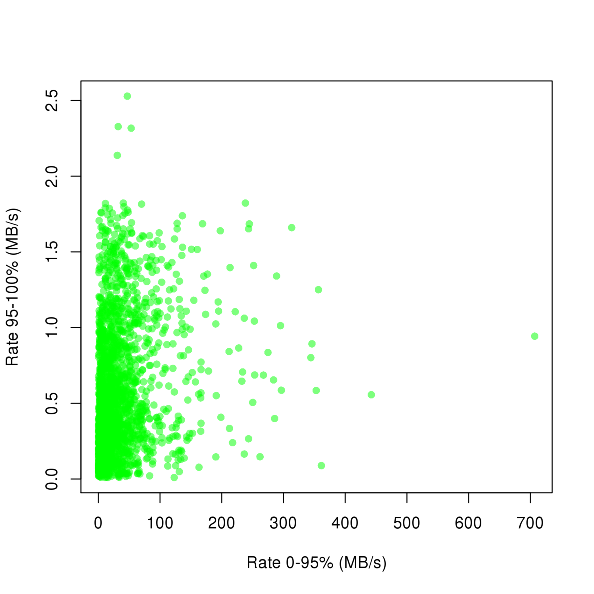
\includegraphics{Figures/figure-51.pdf}
\caption{}\label{fig:figure-5.1}
\end{figure}

\begin{figure}[htp]
\centering
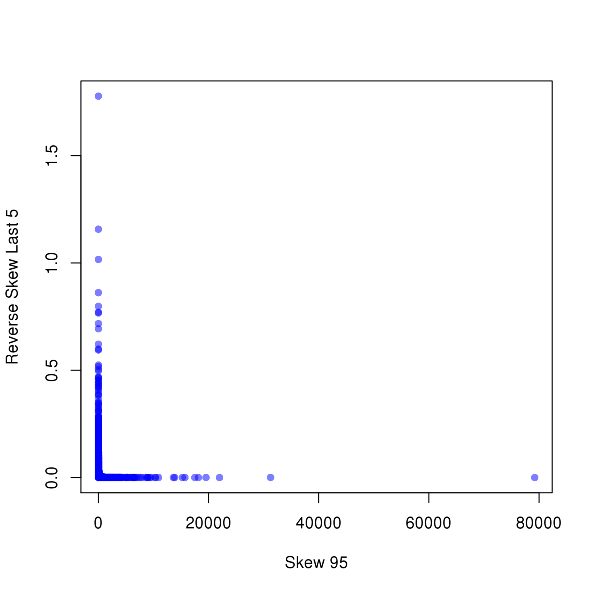
\includegraphics{Figures/figure-52.pdf}
\caption{}\label{fig:figure-5.2}
\end{figure}

When the CMS PhEDEx team investigated the underlying reasons for file
production failures, it was observed that it is mainly due to
transient storage problems. This also explains why only a few files
are affected from this issue. As T1s have more reliable storage
systems, it is mostly T2s that are particularly exposed to this source
of latency, as can be seen in figure~\ref{fig:figure-5.3}.

\begin{figure}[htp]
\centering
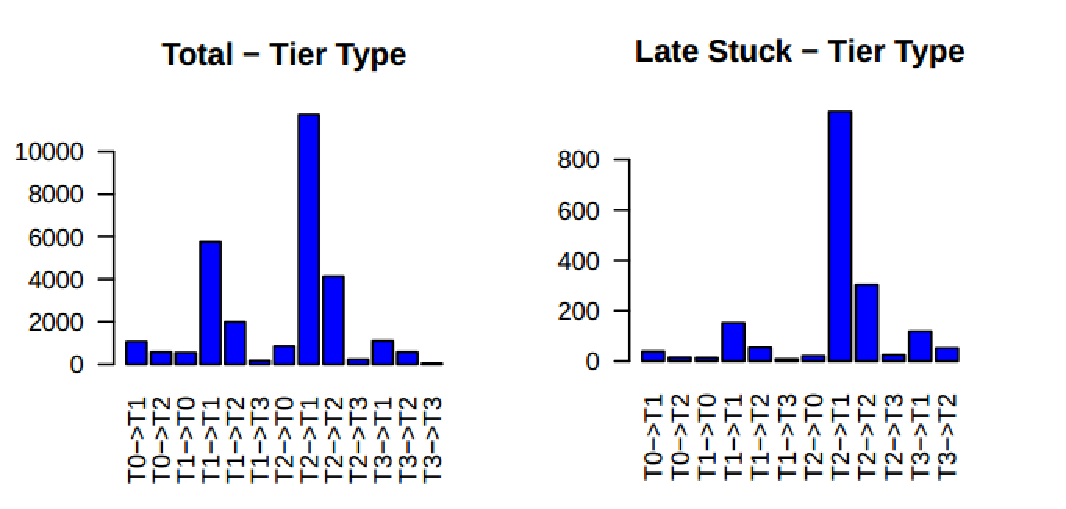
\includegraphics{Figures/figure-53.pdf}
\caption{}\label{fig:figure-5.3}
\end{figure}


Despite the fact that even 99\% of any given sample has already been
transferred to the expected destination, most frequently the
transferred data is useless to CMS jobs until a 100\% transfer
completion is reached. Thus, it is quite important to find the “stuck”
files being the root cause of the latency, and fix the identified
problems as soon as possible. In most cases, solving this problem
requires a manual expert operator intervention, consisting of either
replacing the file (if it has other valid replicas) or otherwise
invalidating it and announcing it as lost.

\section{Latency of blocks that get stuck early}
\label{sec:earlystuck}

The overall CMS production resources consist of a highly
interconnected pool of WLCG sites of different capacities and
belonging to different Tier levels. All of them are actively used in
processing/production activities, and an efficient and closely
monitored data transfer system on this complex topology is
essential. It is not unexpected that, in exploiting this heterogeneous
set of resources over long periods of time, some permanent or
transient errors due to hardware/software problems are
experienced. Although CMS tries hard to detect the problematic sites
in advance and proactively takes measures to use them only if they are
safe both for processing and for data transfers, it is not always
possible to select with 100\% purity on long periods of time a subset
consisting of only sites in perfect shape. Hence, it is expected that
the overall transfer system needs to always deal with a bunch of
problematic sites that should nevertheless be used as either source or
destination of some data transfer tasks. In many of these cases, as
the problem may just be at the infrastructural site level, these kind
of transfers show up as “stuck” in the very beginning, i.e. even in
the transfer of the very first file.

\begin{figure}[htp]
\centering
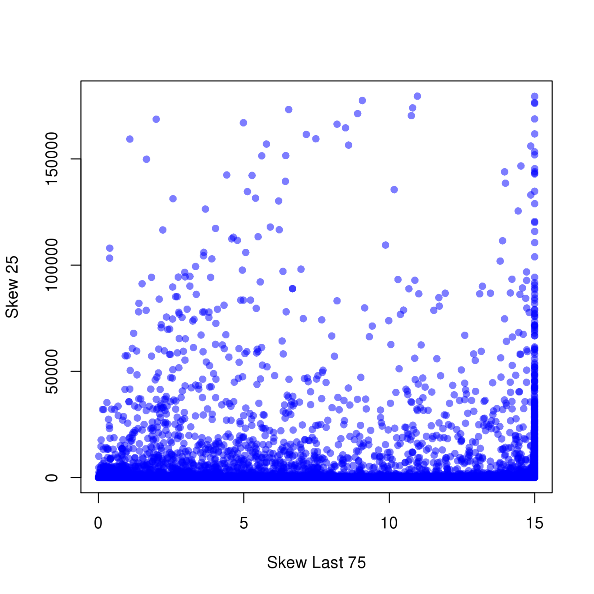
\includegraphics{Figures/figure-72.pdf}
\caption{$Skew_{25}$ versus $SkewLast_{75}$ as defined in
  eq.~\ref{eq:skew} and eq.~\ref{eq:skewlast}. For transfers tagged as
  being ``early-stuck'' according to
  eq.~\ref{eq:early-stuck}.}\label{fig:figure-7.2}
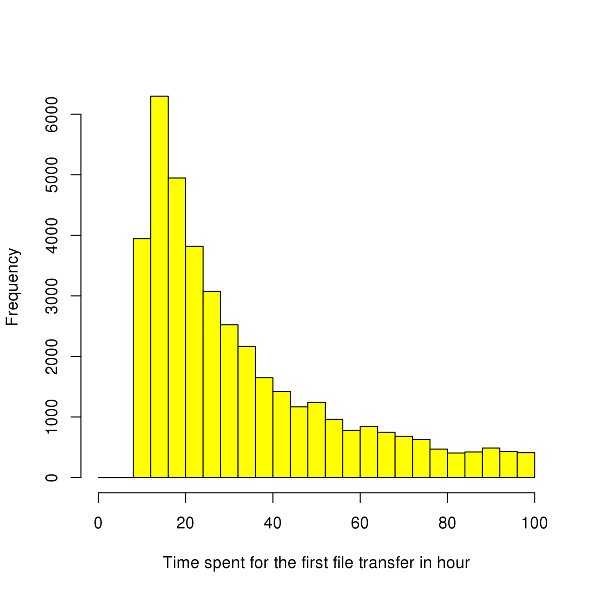
\includegraphics{Figures/figure-71.pdf}
\caption{Frequency histogram of the first file replica time (in hour)
  for the transfers tagged as being ``early-stuck'' according to
  eq.~\ref{eq:early-stuck}.}\label{fig:figure-7.1}
\end{figure}

These transfers are hence reported as stuck at 0\% completion for
hours as shown in fig.~\ref{fig:figure-7.1}, so it is far easier
to detect them with respect to any other latency type.

In addition, $SkewLast_{75}$ values (see eq.~\ref{eq:skewlast}) are
quite small while $Skew_{25}$ (see eq.~\ref{eq:skewlast}) have quite
large values in fig.~\ref{fig:figure-7.2} as expected.

%\begin{figure}[htp]
%\centering

%\end{figure}

The solution, however, is not straight-forward: it might require site
admin intervention at the source/destination site, or even central
operators/experts involvement. The price to pay if not promptly
identified is high: only a quick problem identification, attack and
fix can avoid to pile up delays and additional work load at a later
stage.

\section{Latency of datasets with many small blocks}

In all CMS processing activities, the growth of a CMS dataset to be
intended as a collection of files with specific physics content
happens through the contribution of production efforts by different
WLCG sites supporting the CMS workflows, and in many cases sites
contributing to a dataset are not the final destination where such
dataset is supposed to be stored. Hence, a PhEDEx subscription is made
to a tape endpoint and possibly to some disk endpoints to gather all
produced data into the needed places according to CMS
policies. However, some of the blocks might be located at a
problematic site that can cause latency in dataset level transfers.

The underlying problem can be missing/corrupt files, or storage
related problems as mentioned in other latency types.



\par
\section*{References}

\begin{thebibliography}{1}

\bibitem{CompModel}
%  CMS computing : Technical Design Report {\it CERN-LHCC-2005-023}
  Grandi C, Stickland D and Taylor L 2005 The CMS Computing Model {\it CERN-LHCC-2004-35/G-083, CMS note 2004-031}

\bibitem{PhEDEx}
  Egeland R, Wildish T and Metson S 2008 Data transfer infrastructure for CMS data taking,  {\it XII Advanced Computing and Analysis Techniques in Physics Research (Erice, Italy: Proceedings of Science)}

\end{thebibliography}


\end{document}
